Deep neural networks are often thought of as ``black boxes'' that are
easy to train but difficult to intepret. Interpreting the results
obtained using these techniques may indeed be more challenging than
getting the results themselves. This difficulty of interpretation
sometimes leads to the suspiction that the neural network learns
artifacts in the data that correlate with the target results but are
not meaningful on any datasets other that those, chosen for training and evaluation.
%
In this section we attempt to show that our network learns relevant
description of a protein structure and can successfully rank decoys in the 3DRobot dataset.

First, we identify the regions of a structure that are responsible for
an increase of its score (a \emph{decrease} in its quality). If the
network has learned intepretable features of the data, we expect this
analysis to show that the regions responsible for the poor quality of
a decoy structure are those in which it deviates from the native
structure.
%
We use the Grad-CAM analysis technique proposed by Selvaraju et
al.~\cite{selvaraju2016grad}. The key idea of this technique is to
compute the gradient of the model output with respect to the output of a certain layer (``activations'' of the layer) 
and take the sum of these activations weighted by the gradient.
This highlights output regions of that layer that are both strongly
activated and highly influential on the output.
The weighted layer output is then upscaled to the same size as the input of the network. 
It indicate which parts of the input contribute the most to the gradient of the network output.
In our case we choose the ReLU layer 10, for which
the output size is $25\times 25\times 25$.
We tested the method on the outputs of the neighboring layers and
layer 10 represents the best tradeoff between interpretability and
coarseness.

An example of the Grad-CAM output is given in Fig.~\ref{Fig:GradCAMT0776}.
In line with our scoring procedure, we perform the Grad-CAM analysis
by uniformly sampling 90 rotations and translations of the decoy. We
obtain the Grad-CAM output for each transformation and
project it onto the atoms of the decoy. 
Figure~\ref{Fig:GradCAMT0776} shows two representations of Grad-CAM result 
(for decoy Distill\_TS3 of target T0776): the
projection of the map onto the atoms of the decoy, represented as a
color-coded value on the cartoon rendering of the structure, and the
projection onto a 3D grid, represented as an isosurface. The
isosurface of Fig.~\ref{Fig:GradCAMT0776} is a hollow shell containing
most of the solvent exposed region of the decoy, which indicates that
the network enforces packing: any increase in the atomic density
around the well-packed core decreases the quality of the decoy.
%
We also found that the weighted layer outputs are mostly zero for
structures close to the native ones (results not shown), despite the
fact that no gradient information was included in the training
procedure.

Figure~\ref{Fig:GradCAMT0776_more} shows the color-coded
values of the Grad-CAM result for the four decoys of target T0776.
We see, that the position of the N-terminal alpha-helix (which was not present in the target native structure) 
strongly influences the predictions. In case of the decoys Distill\_TS3 and 3D-Jigsaw-V5\_1\_TS2 our algorithm 
highlights this helix as the one contributing to the quality. On the other hand FALCON\_TOPO\_TS3 places this helix 
differently. This placement also better corresponds to placement of the preceeding loop in the native structure.

\begin{figure}[H]
    \centering
    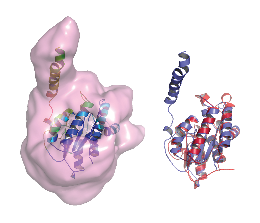
\includegraphics[width=0.5\linewidth]{Fig/FigT0776.eps}
%
    \caption{Left: The output of the Grad-CAM algorithm for the layer 10 on
    candidate structure Distill\_TS3 of target T0776. The isosurface
    shows the scaled outputs at the two-sigma level. The intensities
    of the outputs at the positions of the protein atoms are
    color-coded on the cartoon rendering of the structure, from blue
    (low intensity) to red (high intensity). Right: Cartoon
    representation of the Distill\_TS3 decoy structure (in blue)
    aligned to the native structure (in red).}
    \label{Fig:GradCAMT0776}
\end{figure}

\begin{figure}[H]
    \centering
    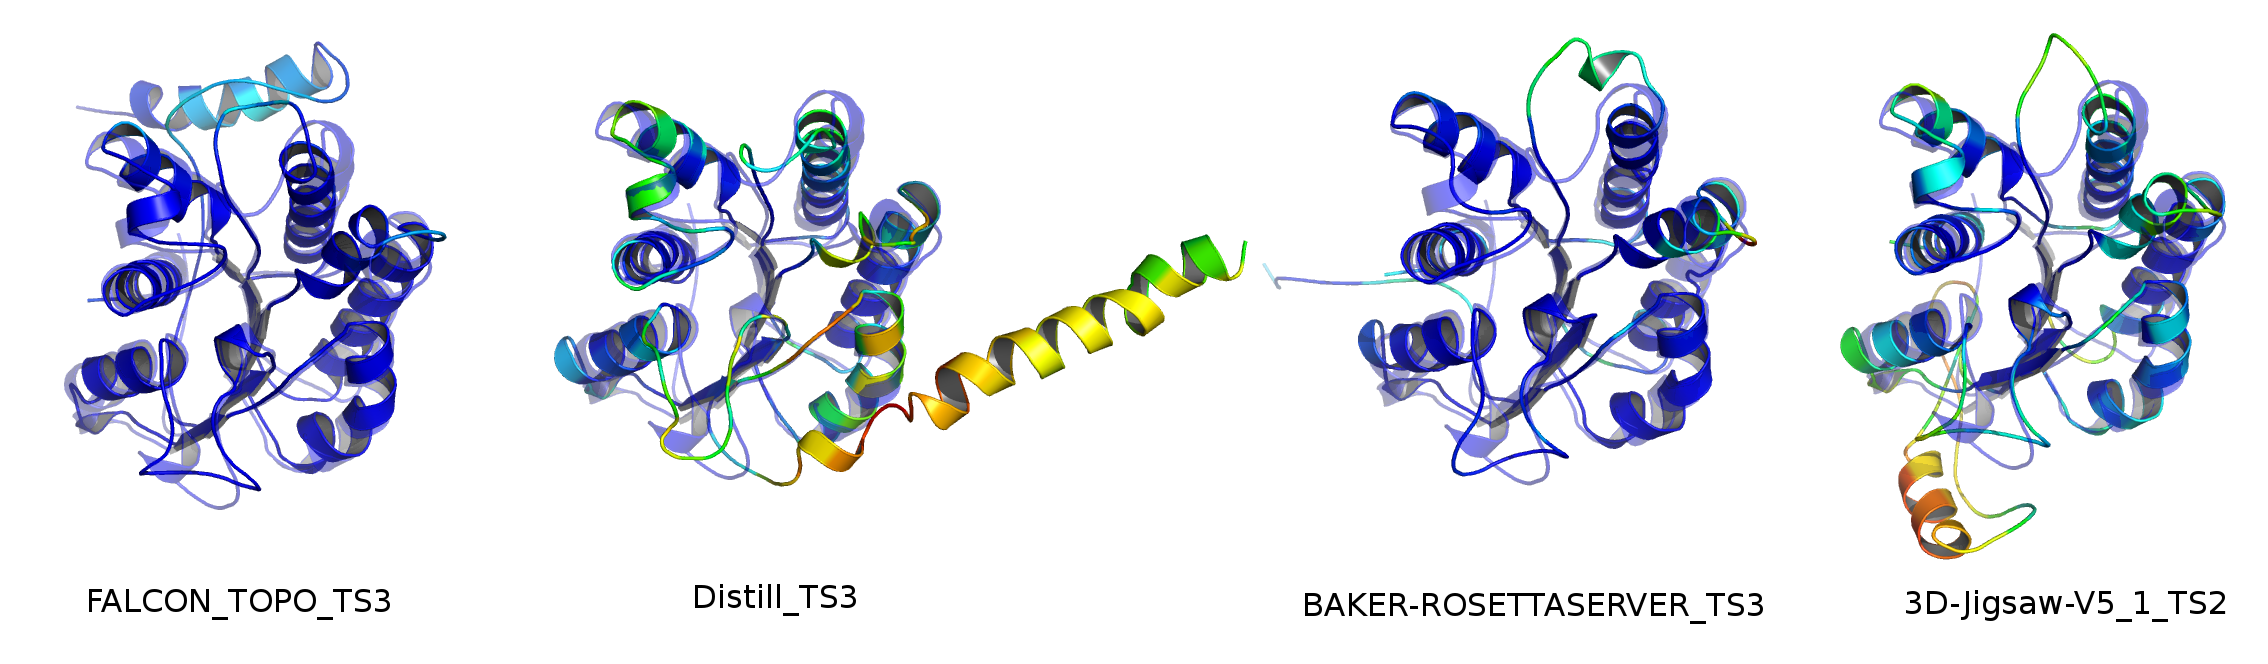
\includegraphics[width=\linewidth]{Fig/T0776.eps}
%
    \caption{The output of the Grad-CAM algorithm for the layer 10 of the network
    projected onto the atoms of the decoys. Each decoy is aligned to
    the native structure, shown as a transparent, blue cartoon.}
    \label{Fig:GradCAMT0776_more}
\end{figure}

To verify that the network we trained does not rely on artifacts in
the data to rank decoys, we have assessed its performance on a second,
independent dataset generated by the 3DRobot
algorithm \cite{deng20163drobot}. The decoys generated by this
algorithm are uniformly distributed within RMSD range of $[0; 12\AA]$
of the native structure and are optimized for the number of hydrogen
bonds and compactness.

The dataset consists of 300 decoys for each of the 200 non-redundant proteins. The proteins were 
selected from the PDB database with less than 20\% pair sequence identity, containing 48 $\alpha$, 
40 $\beta$ and 112 $\alpha/\beta$ signle-domain proteins with length from 80 to 250 residues. 
The absolute Pearson $R$ coefficient averaged per-target over all the
targets in this benchmark was $0.85$. Spearman $\rho$ coefficient
and Kendall $\tau$ coefficient were $0.83$ and $0.64$, respectively.
Representative examples of score versus GDT\_TS plots are shown in
Fig.~\ref{Fig:3DRobotBenchmark}.  We see, that the MQA method devised
in this work successfully ranks unrelated datasets.
\begin{figure}[H]
    \centering
    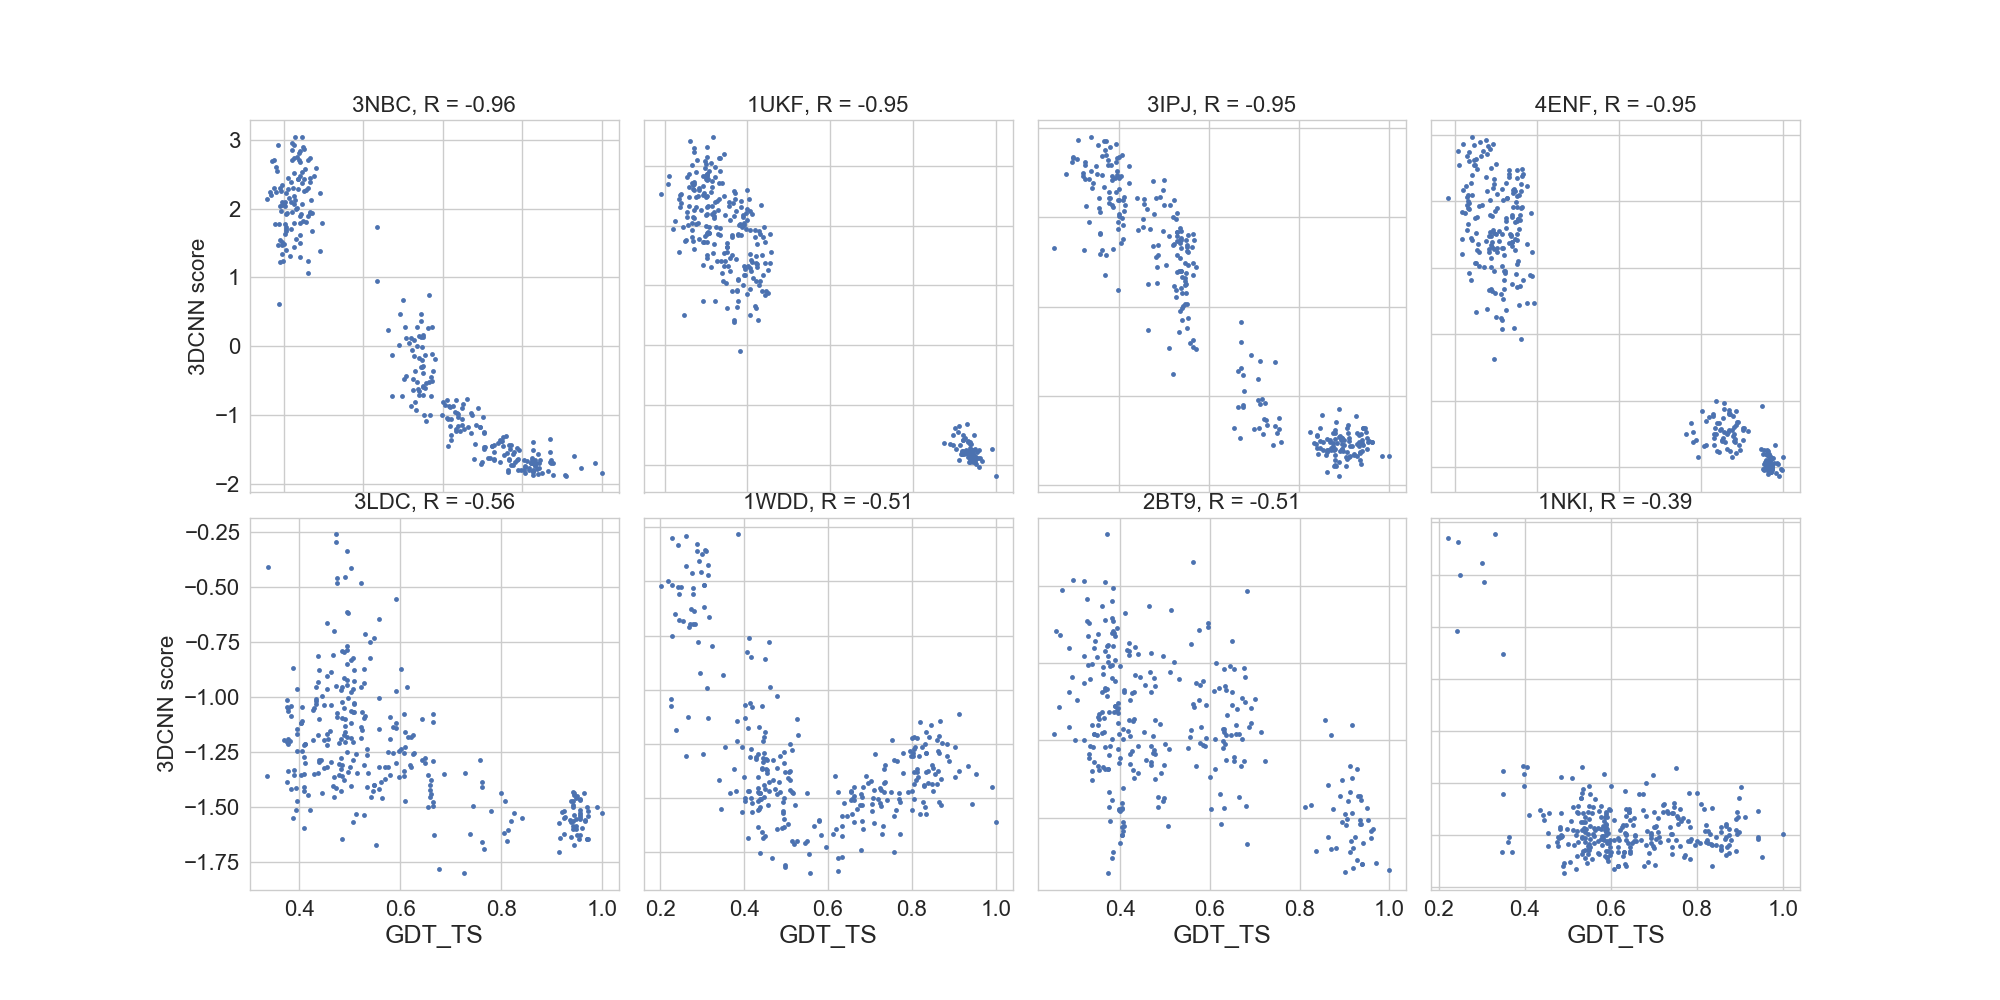
\includegraphics[width=\linewidth]{Fig/3DRobot_set_sFinal_funnels.eps}
%
    \caption{The plots of score versus GDT\_TS for four best correlated targets and four
    least correlated targets in the 3DRobot benchmark.}
    \label{Fig:3DRobotBenchmark}
\end{figure}
